%!TEX root = report.tex
\chapter{WebApp for Active Delay Warning}
\label{ch:mobile_app}

\par We designed a web application to demonstrate the potential use of our API data service. It allows users to search for nearby bus stops, view the available routes and live bus arrival times. For each route, the user can view the historical, current and reference bus travel time to reach each downstream bus stop.

\section{Implementation}
\subsection{AugularJS Framework}
\par We chose to use the AngularJS Framework \cite{angularjs} with UI Bootstrap \cite{bootstrap} to build the frontend of the application. This was because AngularJS employs a clear Model-View-Controller structure, and has a wide range of packages to build extensions with.

\subsection{Development \& Deployment Pipeline}
\par We used Yeoman \cite{yeoman}, a web application scaffolding tool, to organise and manage scripts and files. We also used Grunt \cite{grunt}, a Javascript task runner to manage the build and delopment process.

\par For deployment, we created a Grunt task to run tests, minify the javascript files, and copy the minified version to the production server.

\section{Frontend Walkthrough}
\par We deployed the frontend web to \url{http://delay.doc.ic.ac.uk/}.

\subsection{Landing Page}
\par The map will be centered at the current location of the device. If the current location is not available, then the default map centered on London will be loaded (Figure \ref{fig:landing_page}).

\begin{figure}
\centering
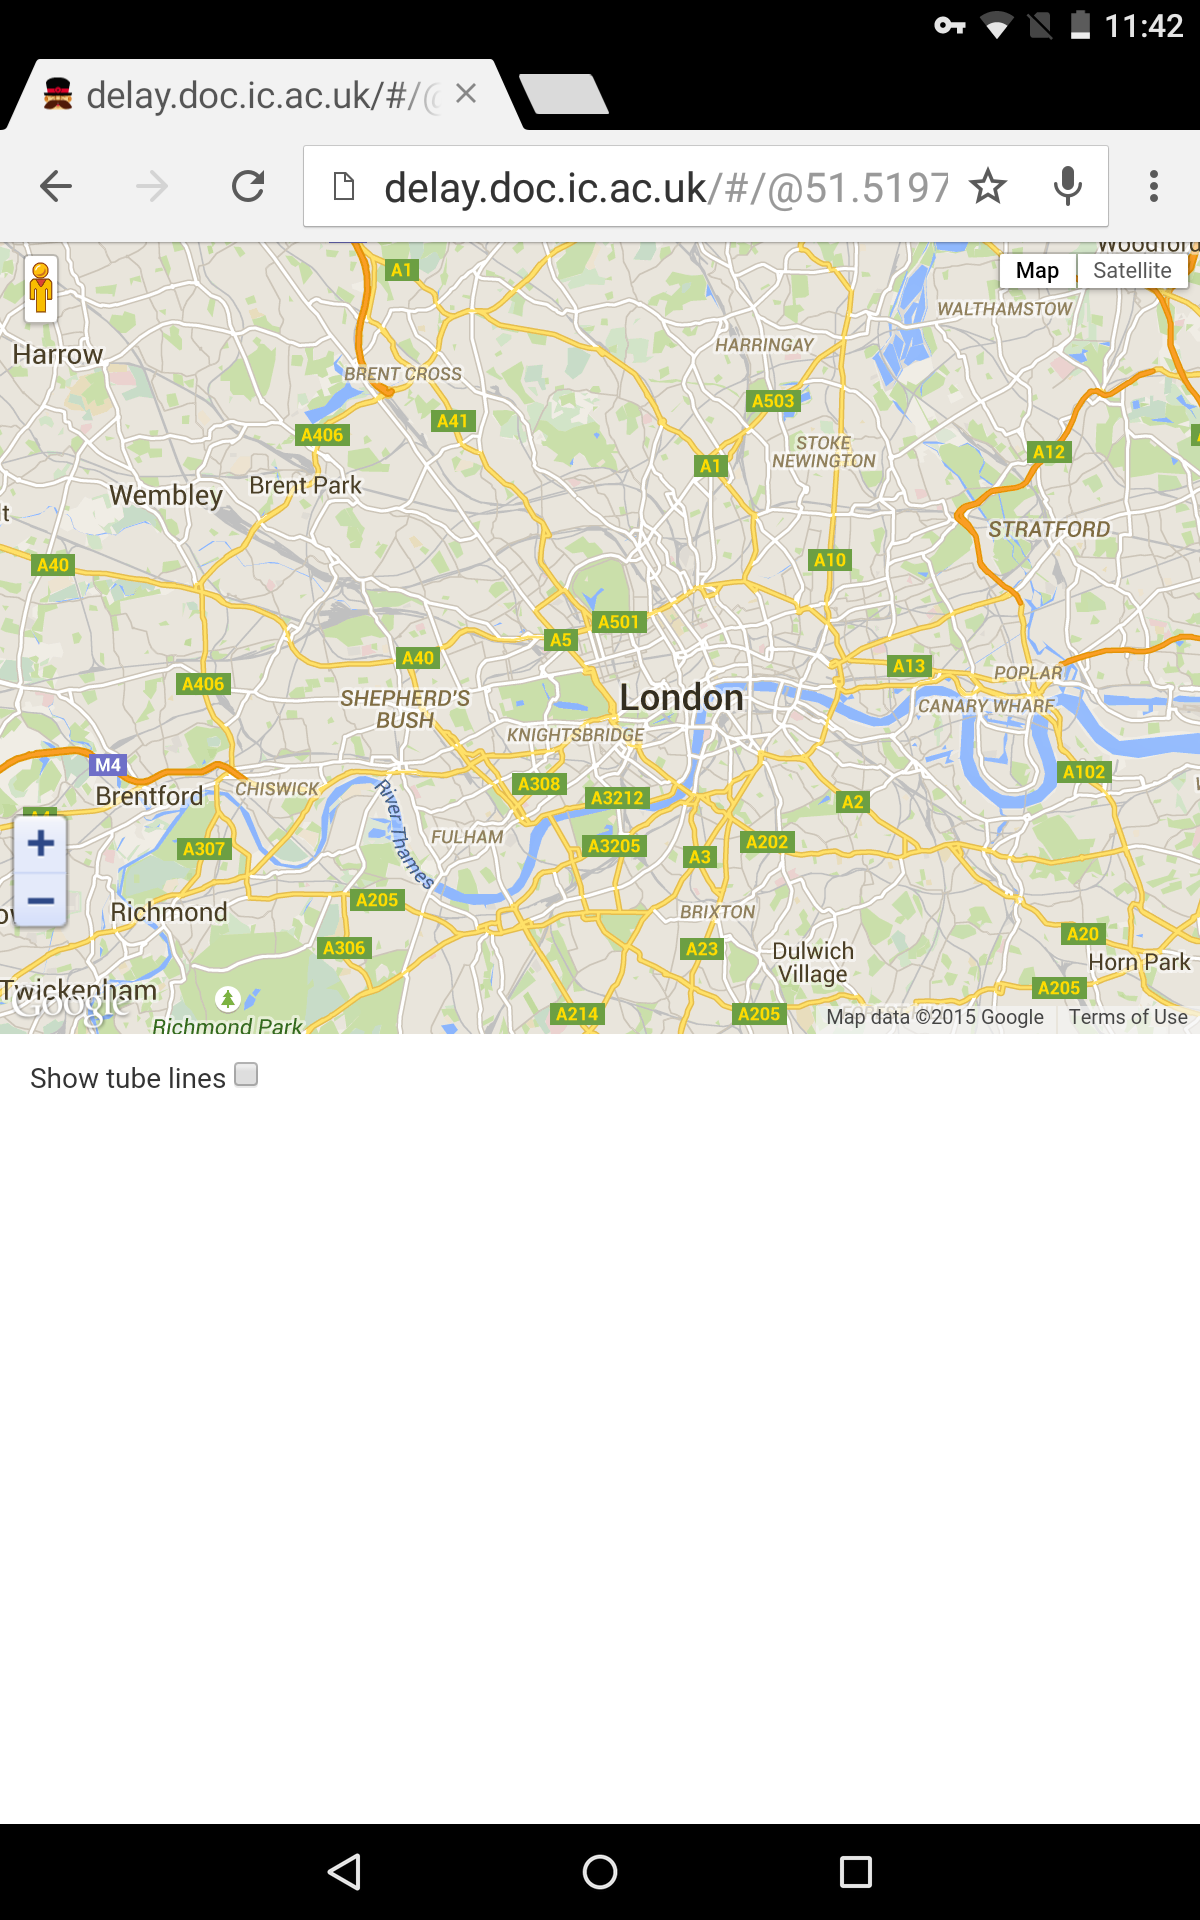
\includegraphics[width=0.8\textwidth]{figures/landing_page.png}
\caption{\label{fig:landing_page} Web Application Langding Page}
\end{figure}

\subsection{Nearby Bus Stops Arrival}
\par A click on the map will place a grey location marker and make a request to search for the nearby bus stops within a given radius. The default radius is 100 meters. A list of the nearby bus stops and the routes available at each stop will be shown, with the \acrshort{tfl} bus arrivals predictions shown(Figure \ref{fig:clicked_view}).

\begin{figure}
\centering
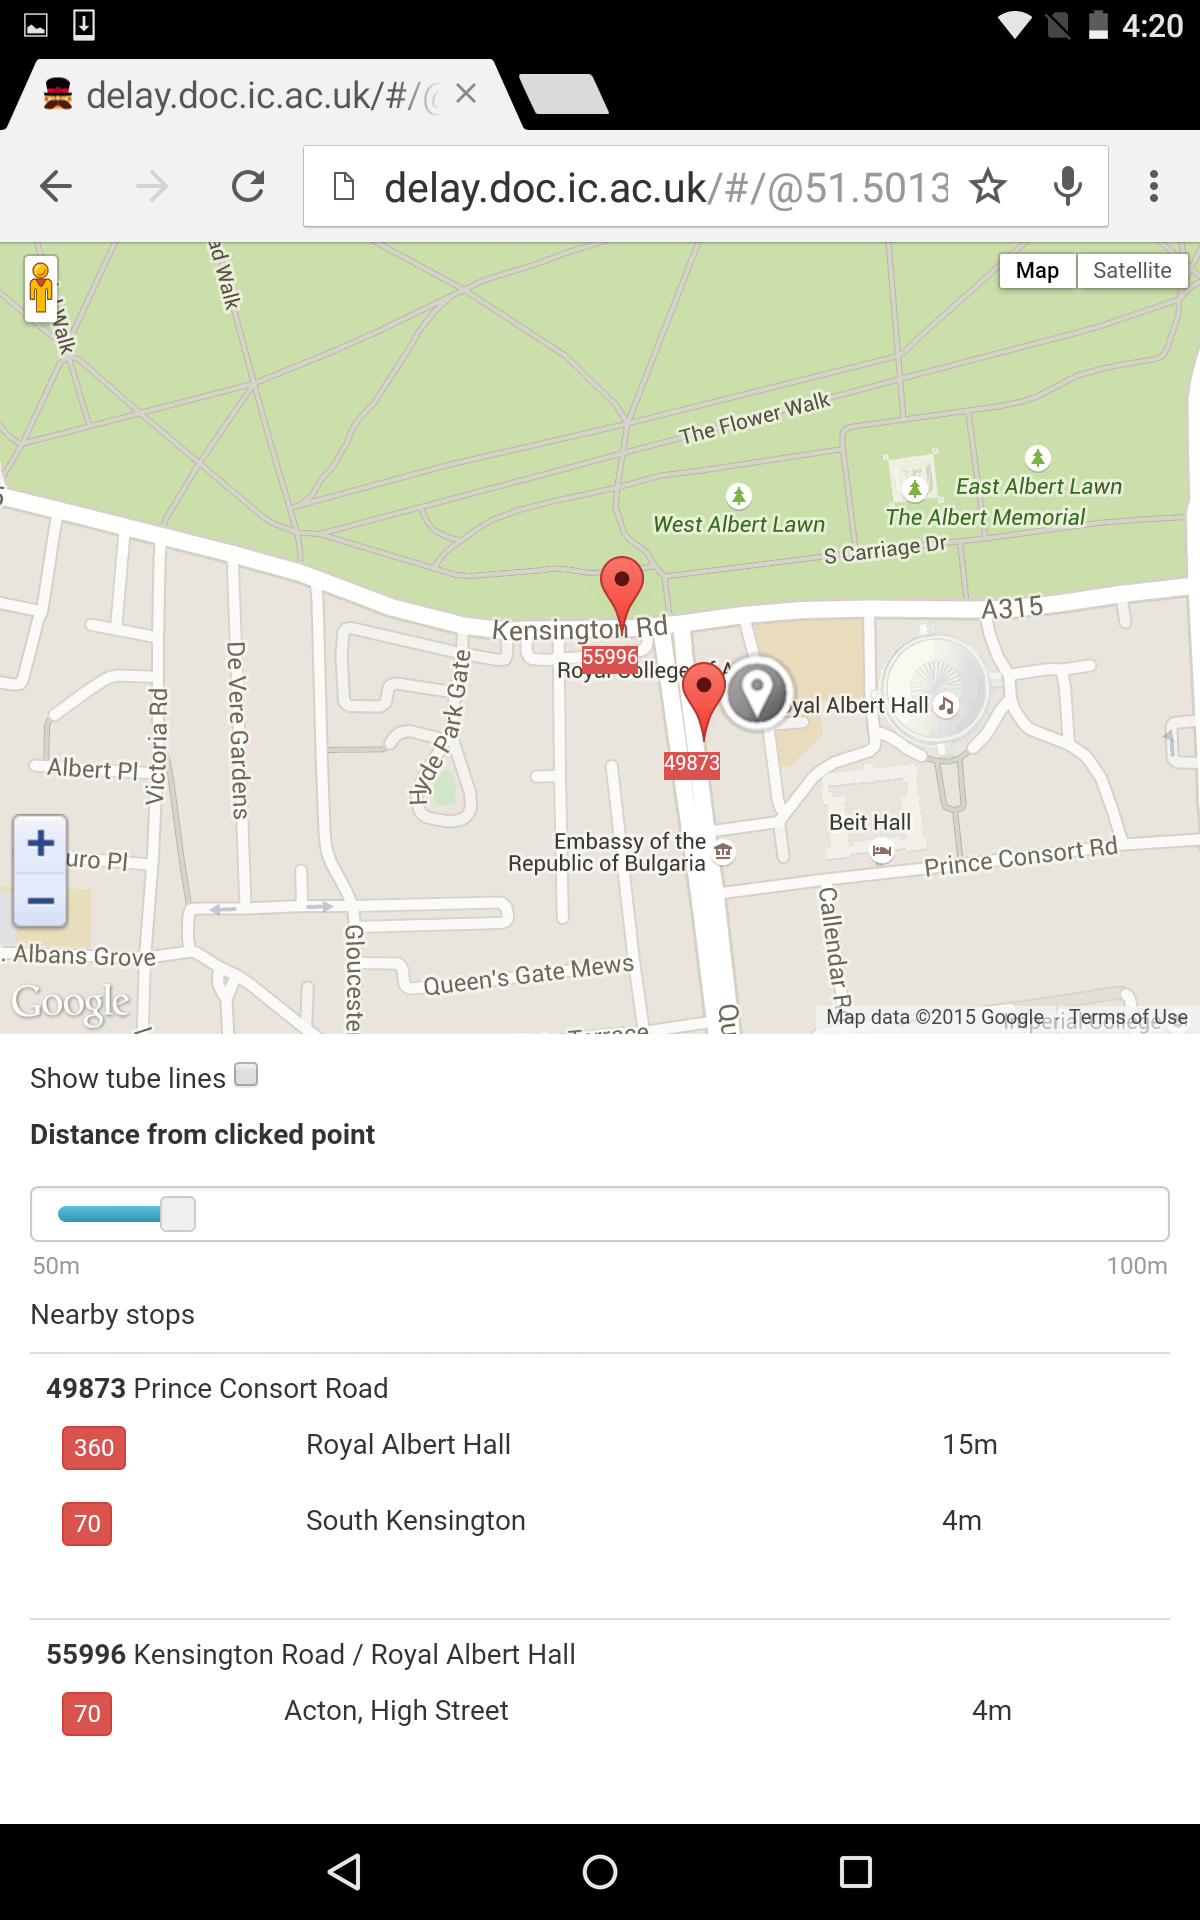
\includegraphics[width=0.8\textwidth]{figures/clicked_view.png}
\caption{\label{fig:clicked_view} Web Application Nearby Bus Stops}
\end{figure}

\subsection{Bus Delay Predictions}
\par We could check the historical, current, and reference travel time to each downstream stops by selecting a specific route for details. There is likely delay when the current bus travel time is more than the reference bus travel time. For example, in Figure \ref{fig:timetable_view}, there is a slight delay for bus 70 from Kensington Road.


\begin{figure}
\centering
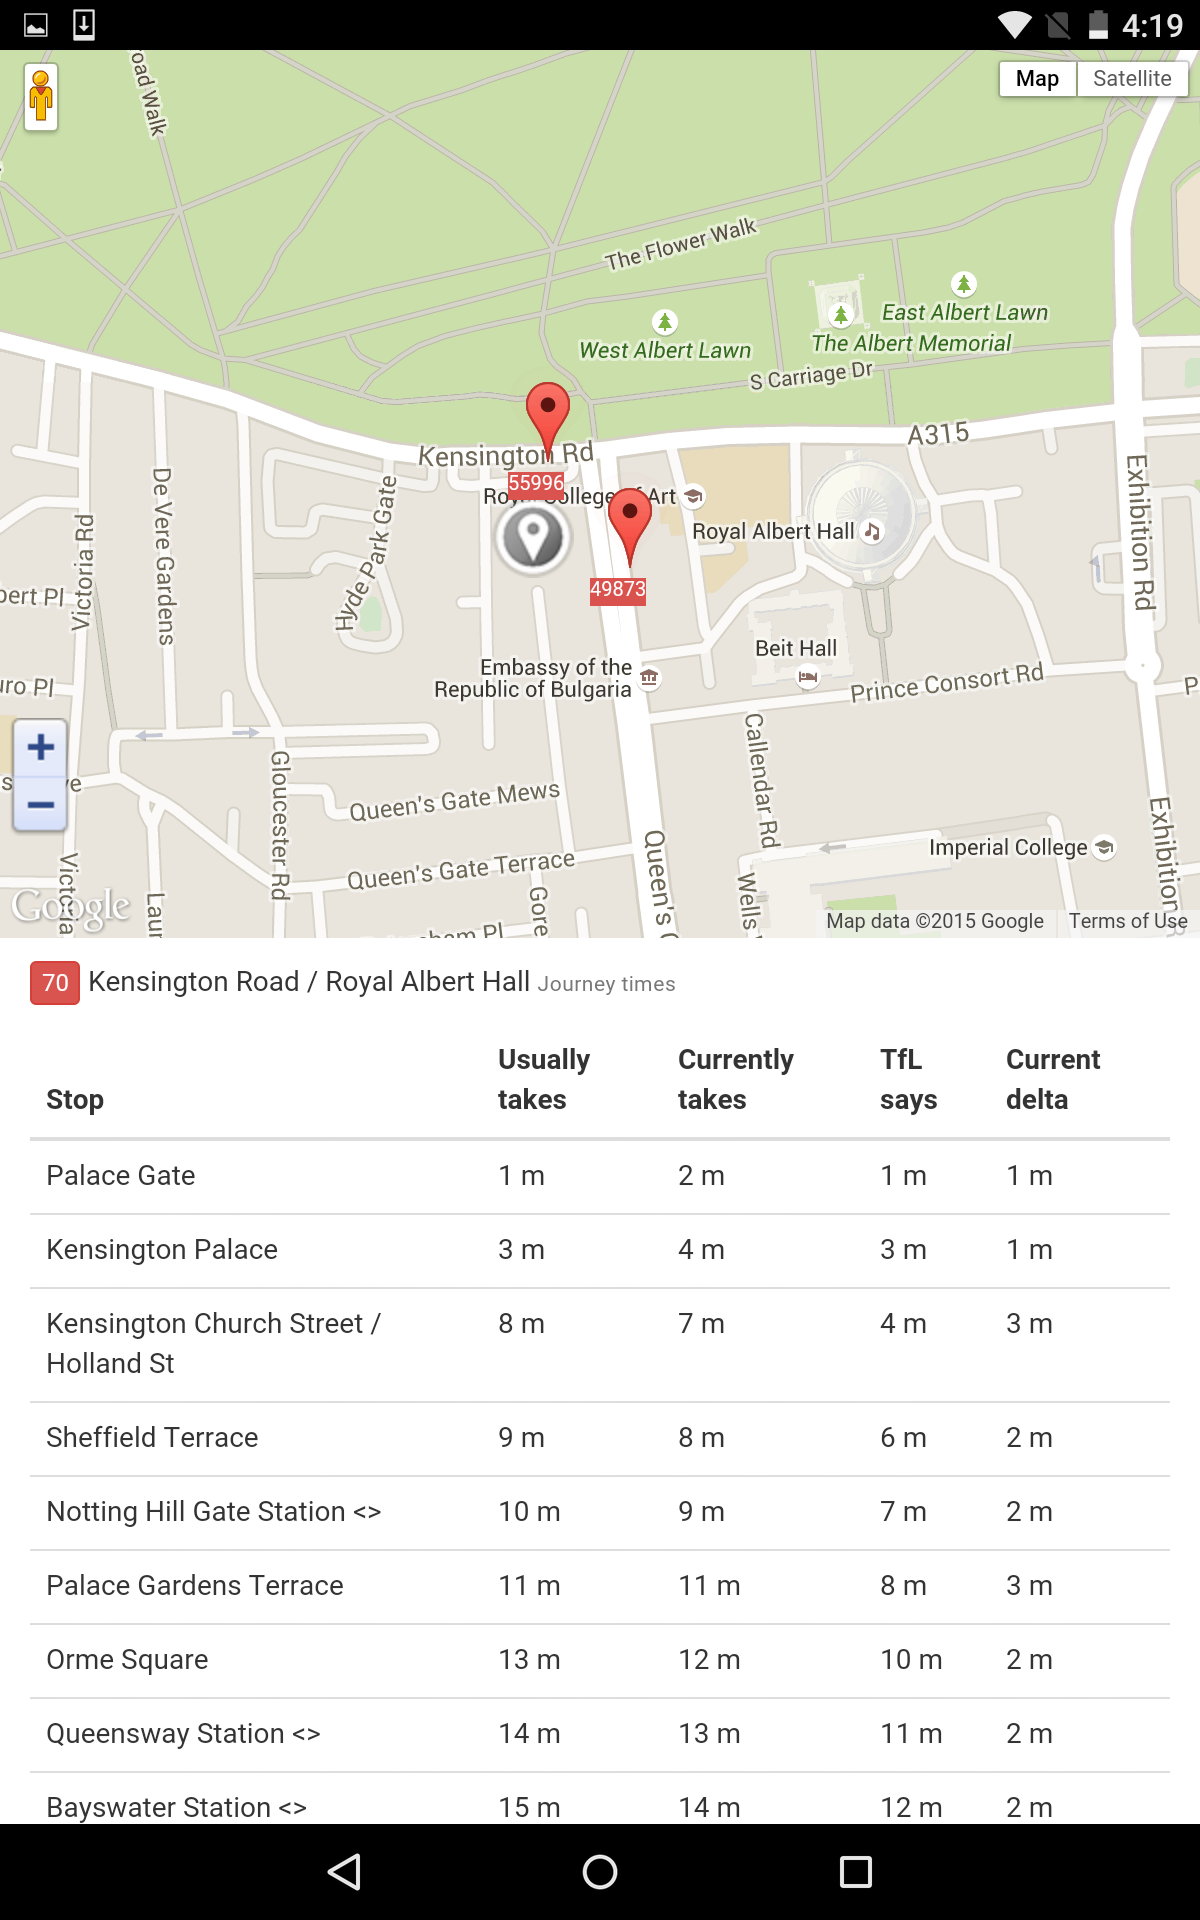
\includegraphics[width=0.8\textwidth]{figures/timetables.png}
\caption{\label{fig:timetable_view} Web Application Timetables for a Route}
\end{figure}

\section{Summary}
\par The web application shows how the delay prediction data service could be used to inform users of potential delays in buses arriving at any downstream stops on a selected route. This will help bus passengers to make informed decisions when choosing travel mode and bus routes to save time.

